{\fontfamily{cmss}\selectfont

\begin{tabular}{m{0.33\linewidth}m{0.3\linewidth}m{0.24\linewidth}}
\parbox{\linewidth}{
  {\textcolor{gray!50}{\small\textit{prose-report}}}
  
  \vspace{0.2cm}
  {\LARGE \VAR{target}}

  \vspace{-0.1cm}
  {\footnotesize\textit{\VAR{description}}}

  \boxtitle{NIGHT}
  \mbox{\hspace{-0.7cm}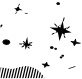
\includegraphics[width=\linewidth + 0.7cm]{summary/figures/stars}}
  \vspace{-1cm}\newline

  {\bgroup
  \def\arraystretch{1.2}% 
  \tiny
  \rowcolors{1}{white}{gray!8}
  \roboto
  \begin{tabular}{|m{0.45\linewidth}|m{0.45\linewidth}|}
      \BLOCK{for name, value in obstable}
          \hline
          \textcolor{black!50}{\VAR{name}} & \VAR{value}\\
      \BLOCK{endfor}
     \hline
  \end{tabular}
  \egroup}

  \boxtitle{PSF}
  \mbox{\hspace{-0.92cm}\includegraphics[width=\linewidth + 0.92cm]{summary/figures/psf}}
} & \hspace{0.7cm}\parbox{\linewidth}{
  \boxtitle{LIGHTCURVE}
  \mbox{\hspace{-1cm}\includegraphics[width=\linewidth + 1cm]{summary/figures/lightcurve}}
  % To be added in future
  % {\centering{\footnotesize model: $f = c + fwhm^2 + sky^2 + T + \epsilon$}}

  \boxtitle{RAW}
  \mbox{\hspace{-0.8cm}\includegraphics[width=\linewidth + 0.8cm]{summary/figures/raw}}
} & \hspace{1.5cm}\parbox{\linewidth}{
  
\boxtitle{SYSTEMATICS}
  \mbox{\hspace{-0.9cm}\includegraphics[width=\linewidth + 0.9cm]{summary/figures/systematics}}
  
  \vspace{-0.2cm}
  \boxtitle{COMPARISON STARS}
  \mbox{\hspace{-0.9cm}\includegraphics[width=\linewidth + 0.9cm]{summary/figures/comparison}}
} \\
\end{tabular}

\newpage

\begin{flushleft}
\begin{tabular}{m{0.97\linewidth}}
\parbox{\linewidth}{

  \boxtitle{ADDITIONAL NOTES}
  \mbox{ \vbox{ \vspace{1cm}\textbf{Goal of the observation}: ... \\
  \begin{itemize}
      \item TOI/TIC ... has been observed with ... on the night of UTC ... in the ... filter.
      \item The transit is/is not detected on the target star which is labeled ... on the stack image and with a depth of about ... ppt. 
      \item The transit timing ... .
      \item The target star light curve has been detrended for ... . 
      \item ... stars are used for comparison, all of them flat and of similar brightness as the target. 
      \item Weather conditions were/were not stable throughout the observation and the moon was at ...\% at ...°.
      \item Comments in TTF before the observation:
  \end{itemize}
   \textbf{Conclusions}: ...
   }}
} 
\end{tabular}
\end{flushleft}

}